\documentclass[tikz,border=2pt]{standalone}
\usetikzlibrary{arrows.meta,positioning,fit,calc}
\definecolor{bfblue}{RGB}{52,109,163}
\definecolor{fporange}{RGB}{213,104,44}
\definecolor{meanpurple}{RGB}{129,89,156}
\definecolor{rewardgreen}{RGB}{57,133,97}
\definecolor{softgray}{RGB}{242,244,247}
\tikzset{
  arrow/.style={-{Latex[length=2mm]}, line width=.7pt, draw=black!65},
  data/.style={draw=black!60, rounded corners=2pt, fill=softgray, align=center, minimum height=7mm, font=\small},
  stage/.style={draw=#1!80!black, rounded corners=3pt, line width=.9pt, fill=#1!7, inner sep=4.5mm},
  process/.style={draw=#1!85!black, rounded corners=2pt, fill=#1!15, align=center, minimum height=9mm, minimum width=26mm, font=\small},
  tinyprocess/.style={draw=#1!85!black, rounded corners=2pt, fill=#1!15, align=center, minimum height=7mm, minimum width=22mm, font=\scriptsize},
  label/.style={font=\bfseries\small, text=#1!80!black}
}
\begin{document}
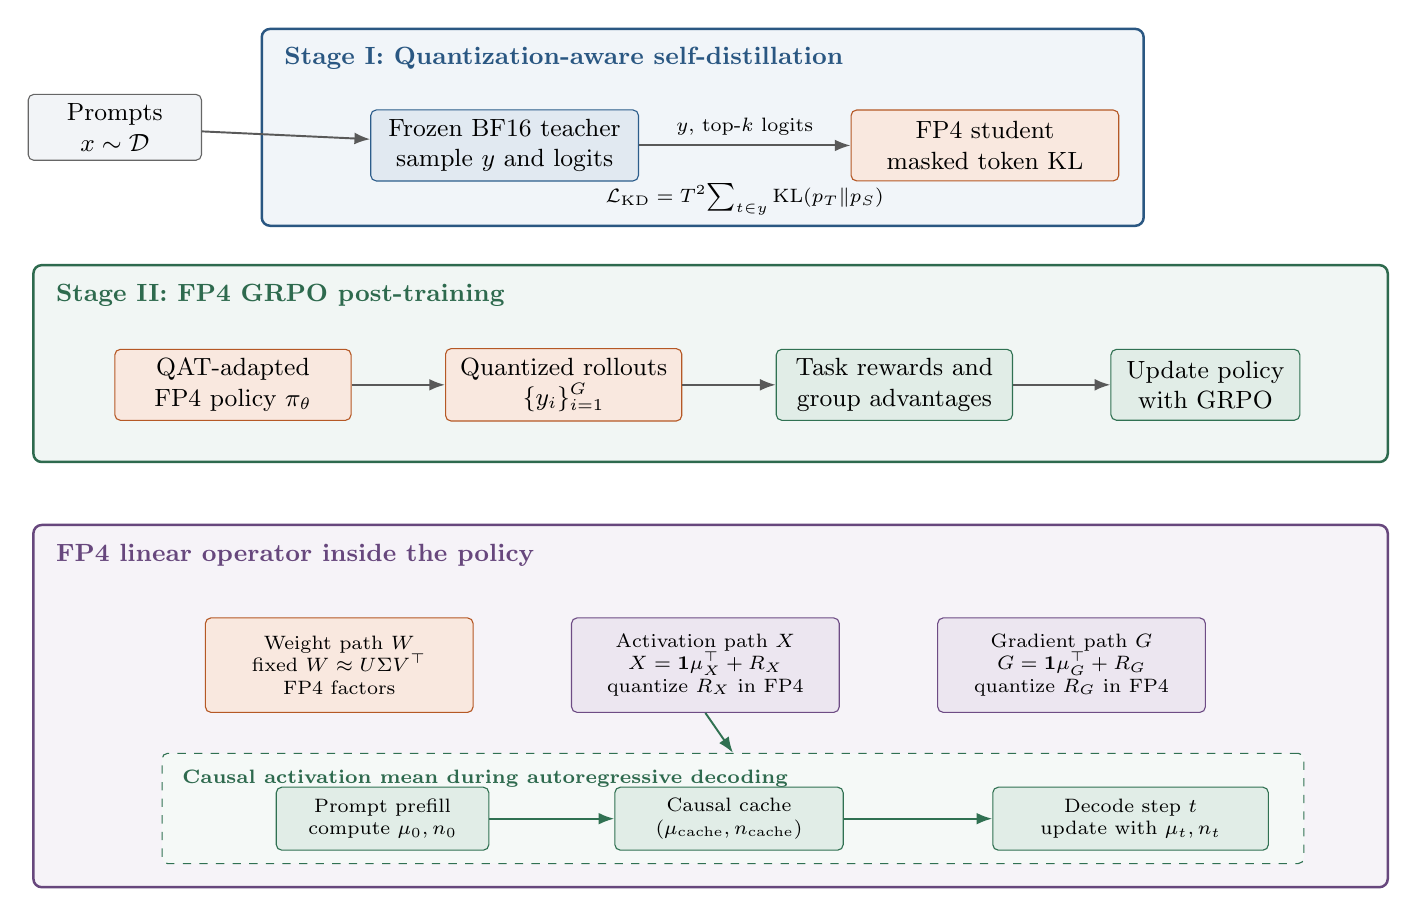
\begin{tikzpicture}[x=1cm,y=1cm]
  % Inputs and QAT stage.
  \node[data, minimum width=22mm] (prompts) at (1.15,5.85) {Prompts\\$x\sim\mathcal{D}$};
  \node[stage=bfblue, minimum width=112mm, minimum height=25mm, anchor=west] (qatbox) at (3.0,5.85) {};
  \node[label=bfblue, anchor=north west] at ($(qatbox.north west)+(0.18,-0.13)$) {Stage I: Quantization-aware self-distillation};
  \node[process=bfblue, minimum width=34mm] (teacher) at (6.1,5.62) {Frozen BF16 teacher\\sample $y$ and logits};
  \node[process=fporange, minimum width=34mm] (student) at (12.2,5.62) {FP4 student\\masked token KL};
  \draw[arrow] (prompts) -- (teacher);
  \draw[arrow] (teacher) -- node[above, font=\scriptsize] {$y$, top-$k$ logits} (student);
  \node[font=\scriptsize] at (9.15,4.93) {$\mathcal{L}_{\mathrm{KD}}=T^2\!\sum_{t\in y}\mathrm{KL}(p_T\Vert p_S)$};

  % GRPO stage.
  \node[stage=rewardgreen, minimum width=172mm, minimum height=25mm, anchor=west] (grpo) at (0.1,2.85) {};
  \node[label=rewardgreen, anchor=north west] at ($(grpo.north west)+(0.18,-0.13)$) {Stage II: FP4 GRPO post-training};
  \node[process=fporange, minimum width=30mm] (policy) at (2.65,2.58) {QAT-adapted\\FP4 policy $\pi_\theta$};
  \node[process=fporange, minimum width=30mm] (rollout) at (6.85,2.58) {Quantized rollouts\\$\{y_i\}_{i=1}^{G}$};
  \node[process=rewardgreen, minimum width=30mm] (reward) at (11.05,2.58) {Task rewards and\\group advantages};
  \node[process=rewardgreen, minimum width=24mm] (update) at (15.0,2.58) {Update policy\\with GRPO};
  \draw[arrow] (policy) -- (rollout);
  \draw[arrow] (rollout) -- (reward);
  \draw[arrow] (reward) -- (update);

  % Quantized linear-layer inset. These are parallel components of the policy,
  % not additional steps in the rollout/update data flow.
  \node[stage=meanpurple, minimum width=172mm, minimum height=46mm, anchor=west] (quant) at (0.1,-1.50) {};
  \node[label=meanpurple, anchor=north west] at ($(quant.north west)+(0.18,-0.13)$) {FP4 linear operator inside the policy};
  \node[tinyprocess=fporange, minimum width=34mm, minimum height=12mm] (weight) at (4.00,-0.98) {Weight path $W$\\fixed $W\approx U\Sigma V^\top$\\FP4 factors};
  \node[tinyprocess=meanpurple, minimum width=34mm, minimum height=12mm] (act) at (8.65,-0.98) {Activation path $X$\\$X=\mathbf{1}\mu_X^\top+R_X$\\quantize $R_X$ in FP4};
  \node[tinyprocess=meanpurple, minimum width=34mm, minimum height=12mm] (grad) at (13.30,-0.98) {Gradient path $G$\\$G=\mathbf{1}\mu_G^\top+R_G$\\quantize $R_G$ in FP4};
  \node[draw=rewardgreen!85!black, dashed, rounded corners=2pt, fill=rewardgreen!5, minimum width=145mm, minimum height=14mm] (actcachegroup) at (9.0,-2.80) {};
  \node[label=rewardgreen, anchor=north west, font=\bfseries\scriptsize] at ($(actcachegroup.north west)+(0.14,-0.10)$) {Causal activation mean during autoregressive decoding};
  \node[tinyprocess=rewardgreen, minimum width=27mm, minimum height=8mm] (prefill) at (4.55,-2.93) {Prompt prefill\\compute $\mu_0,n_0$};
  \node[tinyprocess=rewardgreen, minimum width=29mm, minimum height=8mm] (cache) at (8.95,-2.93) {Causal cache\\$(\mu_{\mathrm{cache}},n_{\mathrm{cache}})$};
  \node[tinyprocess=rewardgreen, minimum width=35mm, minimum height=8mm] (decode) at (14.05,-2.93) {Decode step $t$\\update with $\mu_t,n_t$};
  \draw[arrow, draw=rewardgreen!85!black] (act.south) -- (actcachegroup.north);
  \draw[arrow, draw=rewardgreen!85!black] (prefill) -- (cache);
  \draw[arrow, draw=rewardgreen!85!black] (cache) -- (decode);
\end{tikzpicture}
\end{document}
